This thesis would not have been possible without the input of many along the way.

First, I extend my most sincere gratitude to my advisor Dan Marlow, with whom I have collaborated
during my entire graduate studies.
Dan has been a consistent source of valuable insight and vision for the bigger picture, and
I have benefitted immensely from our conversations about physics and life.
I have seen that performing research occasionally involves
more than understanding the underlying physics,
and Dan's advice in navigating administration has been refreshingly helpful.

I would like to thank the professors in the Princeton Physics Department. In particular
I owe thanks to Chris Tully for discussions related to this thesis and for serving as a second reader,
and to Igor Klebanov and Peter Meyers for serving on committees for my FPO and pre-thesis project.

From my time at Purdue as an undergraduate, I would like to thank my advisor Daniela Bortoletto and
Artur Apresyan. Their influence and patience gave me a strong desire to
see just how deep the rabbit hole goes.
%particle physics was an interesting and worthwhile endeavor.

At CERN, I have had the privilege to work with many talented physicists. In the HggHbb group,
I am indebted to
Olivier Bondu, Maxime Gouzevitch, Chiara Rovelli, Badder Marzocchi, Alexandra Oliveira, and
Amina Zghiche. I have enjoyed defending our colors,
and I hope that Run 2 brings about two Higgs.
%I would especially like to thank Olivier for forcing the use of GitHub in our group,
%ultimately making collaboration easier and more enjoyable.

I owe thanks to many other physicists with whom I have collaborated on other CMS projects, including the
lumi, PLT, W$^\prime$, and VHbb groups. Some of these folks include
Nadia Adam, Adam Hunt, Paul Lujan, Andrzej Zuranski,
Andres Delannoy, Dean Hidas, Andreas Kornmayer, Steve Schnetzer, Bob Stone, 
Sunghyun Chang, Christos Leonidopoulos, Michael Mooney, and Seth Zenz.

I would like to thank the friends over the years of my studies
who have made life as or perhaps more interesting than my physics life,
whether at CERN, Princeton, Purdue, or elsewhere.
Some of these folks include Alex Tuna, Javier Duarte, Kurt Brendlinger, Larry Lee, Sven Rohr,
Aris Alexandradinata, Tim Lou, Eric Smith, Glen Klink, Cody Nelson, and Erik ``Ocho Cinco'' Stahoviak.
Special recognition goes to Tuna, Kurt, Josh Hardenbrook, and Josh Kunkle for contributing
to multiple versions of our CERN relay team -- bestowed with the names Seal Team Six, $\Delta$F,
and Hostage Rescue Team -- and, in turn, creating a true American dynasty.
Heroes are forged in the fires.
%I would like to thank the friends over the years who have made life as or even more interesting
%than my physics life. 
%To those that comprise Centipede, Alex Tuna and Javier Duarte, I hope, nay expect, nay demand,
%that we will run Boston one day.
%To those in the V-card, Tuna and Kurt Brendlinger,
%despite never wanting to use that awful (awesome?) name,
%thanks for accepting me off the streets of Geneva as one of your own.
%To Sven Rohr, I just realized that your future child is perhaps the first infant
%I will take an interest in.
%To those at Princeton, especially Aris Alexandradinata, Tim Lou, and Eric Smith,
%every time I visited we picked up as if I never left.
%To my brahs at the 400, Glen Klink, Cody Nelson, and Erik ``Ocho Cinco'' Stahoviak,
%the last time I visited a portrait studio in the mall was for our family pictures.
%Special recognition goes to Tuna, Kurt, Josh Hardenbrook, and Josh Kunkle for contributing
%to multiple versions of our CERN relay team -- bestowed with the names Seal Team Six, $\Delta$F,
%and Hostage Rescue Team -- and, in turn, creating a true American dynasty.
%Heros are forged in the fires.

La langue française occupait un endroit special pendant le temps que j'ai passé comme doctorat.
Au moment que j'ai su que je déménagerais à Genève, j'ai commencé à l'apprendre avec l'aide de
plusieurs personnes patientes et encourageantes d'abord à Princeton et puis à Genève,
des professeurs ainsi que des amis.
Je remercie Brian Jacobs, Emilie Coquelin, Roberto Daverio, la Croix-Rouge genevoise,
et Liliane Munther. Et je ne veux pas oublier le Jet d'eau et les TPG qui me fascinent
plus qu'ils devraient.

I owe thanks my family whom I have been very fortunate to have by my side through ups and
downs. To my brothers, Craig and Jared, for many years of laughter and fighting, and
to my parents, for always providing a place to call home, I appreciate the constant support
and look forward to what the future has in store for us.
As the great philosopher Vin Diesel once said in a movie I'd wished I'd missed,
``Family is everything.''

Finally, to my fiancée Jigisha Darbha, thanks. %\newline \newline
%Your companionship has provided me many opportunities to grow as a person, and
%when times are rough, you help me to think clearly.
%I am excited that we will soon be officially on the same team.
%As always, I ask for your patience while I slowly learn the language of your ancestors.
%(Thanks to Siriesha for the translation.)
%I look forward to many more adventures in Ireland, India, USA, and wherever else
%public transport may take us.

\vspace{12pt}
\noindent
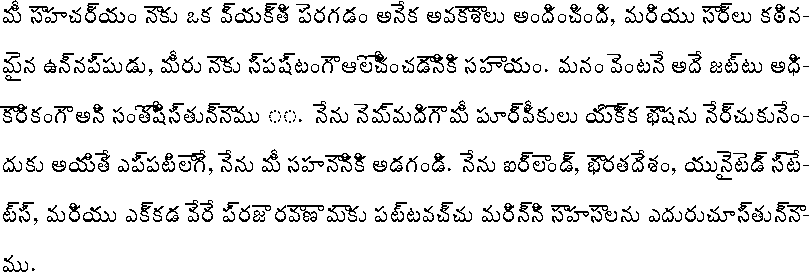
\includegraphics[width=1.0\textwidth]{telugu/thanks.pdf}
%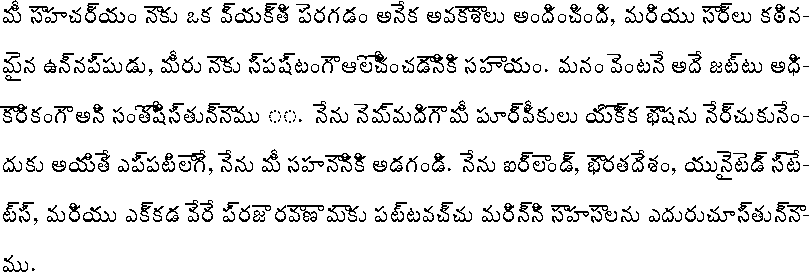
\includepdf{telugu/thanks.pdf}

%\begin{telugu}
%హాయ్ నా పేరు ఫిల్ ఉంది.
%\end{telugu}

\newpage

This material is based upon work supported by the National Science Foundation
Graduate Research Fellowship under Grant No. DGE 1148900
and by the U.S. Department of Energy under Grant No. DOE DE-SC0007968.
